\begin{wrapfigure}{r}{0.45\textwidth} 
	\vspace{-.75em}
	\begin{center}
		\fbox{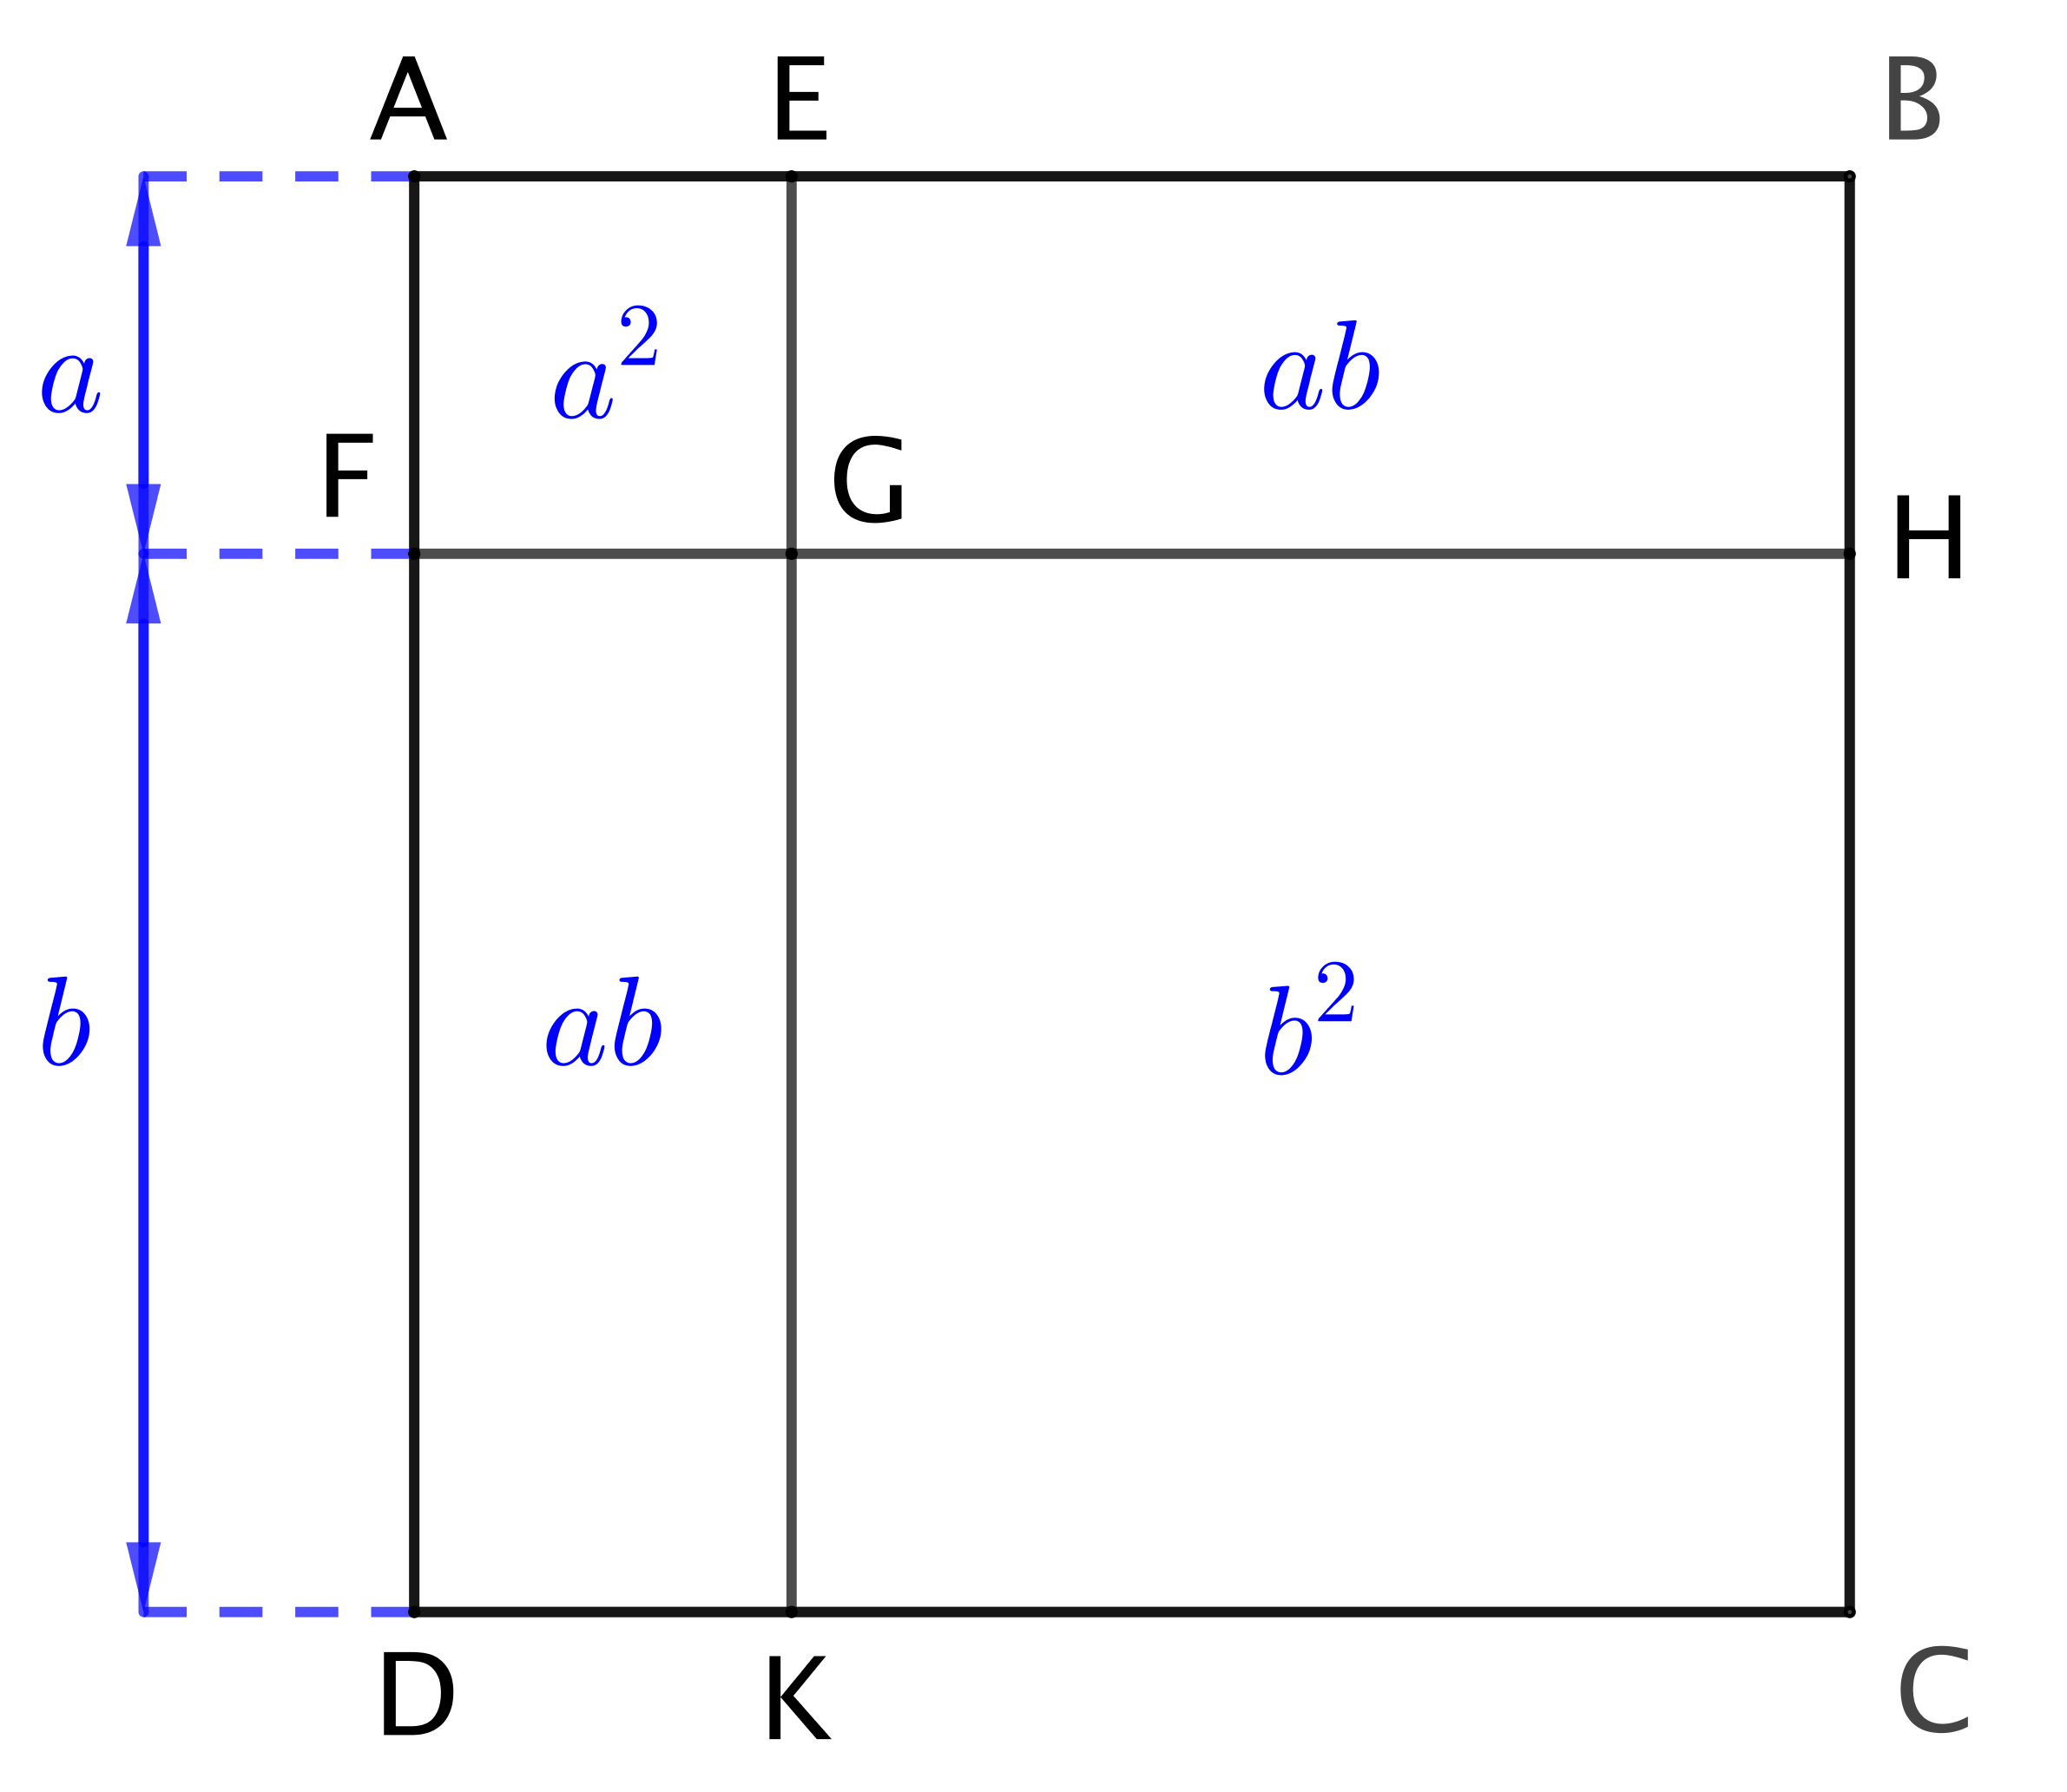
\includegraphics[scale = .7]{/areas-n-identities/(a+b)^2.png}}
	\end{center}
	\vspace{-3em}
\end{wrapfigure} 

Via de simples calculs d'aires, il est très facile de découvrir les identités remarquables suivantes :

\begin{itemize}[label=\small\textbullet]
	\item $(a + b)^2 = a^2 + b^2 + 2ab$

	\item $(a - b)^2 = a^2 + b^2 - 2ab$

	\item $(a + b)(a - b) = a^2 - b^2$
\end{itemize}


\medskip

Par exemple, considérons le dessin ci-contre où $ABCD$ , $AEGF$ et $GHCK$ sont des carrés de côtés respectifs $(a + b)$ , $a$ et $b$ .
Il est évident que nous avons alors $(a + b)^2 = a^2 + b^2 + 2 ab$ mais n'oublions que $a > 0$ et $b > 0$ \emph{(ce sont des contraintes géométriques concrètes)}.


\medskip

Comment passer à $(a + b)^2 = a^2 + b^2 + 2 ab$ pour $a$ et $b$ deux réels de signes quelconques ?
Une première idée est tout simplement de faire une vérification via un calcul algébrique. En résumé, on conjecture géométriquement puis on valide algébriquement.


%\medskip


\begin{wrapfigure}{l}{0.45\textwidth} 
%	\vspace{-.5em}
	\begin{center}
		\fbox{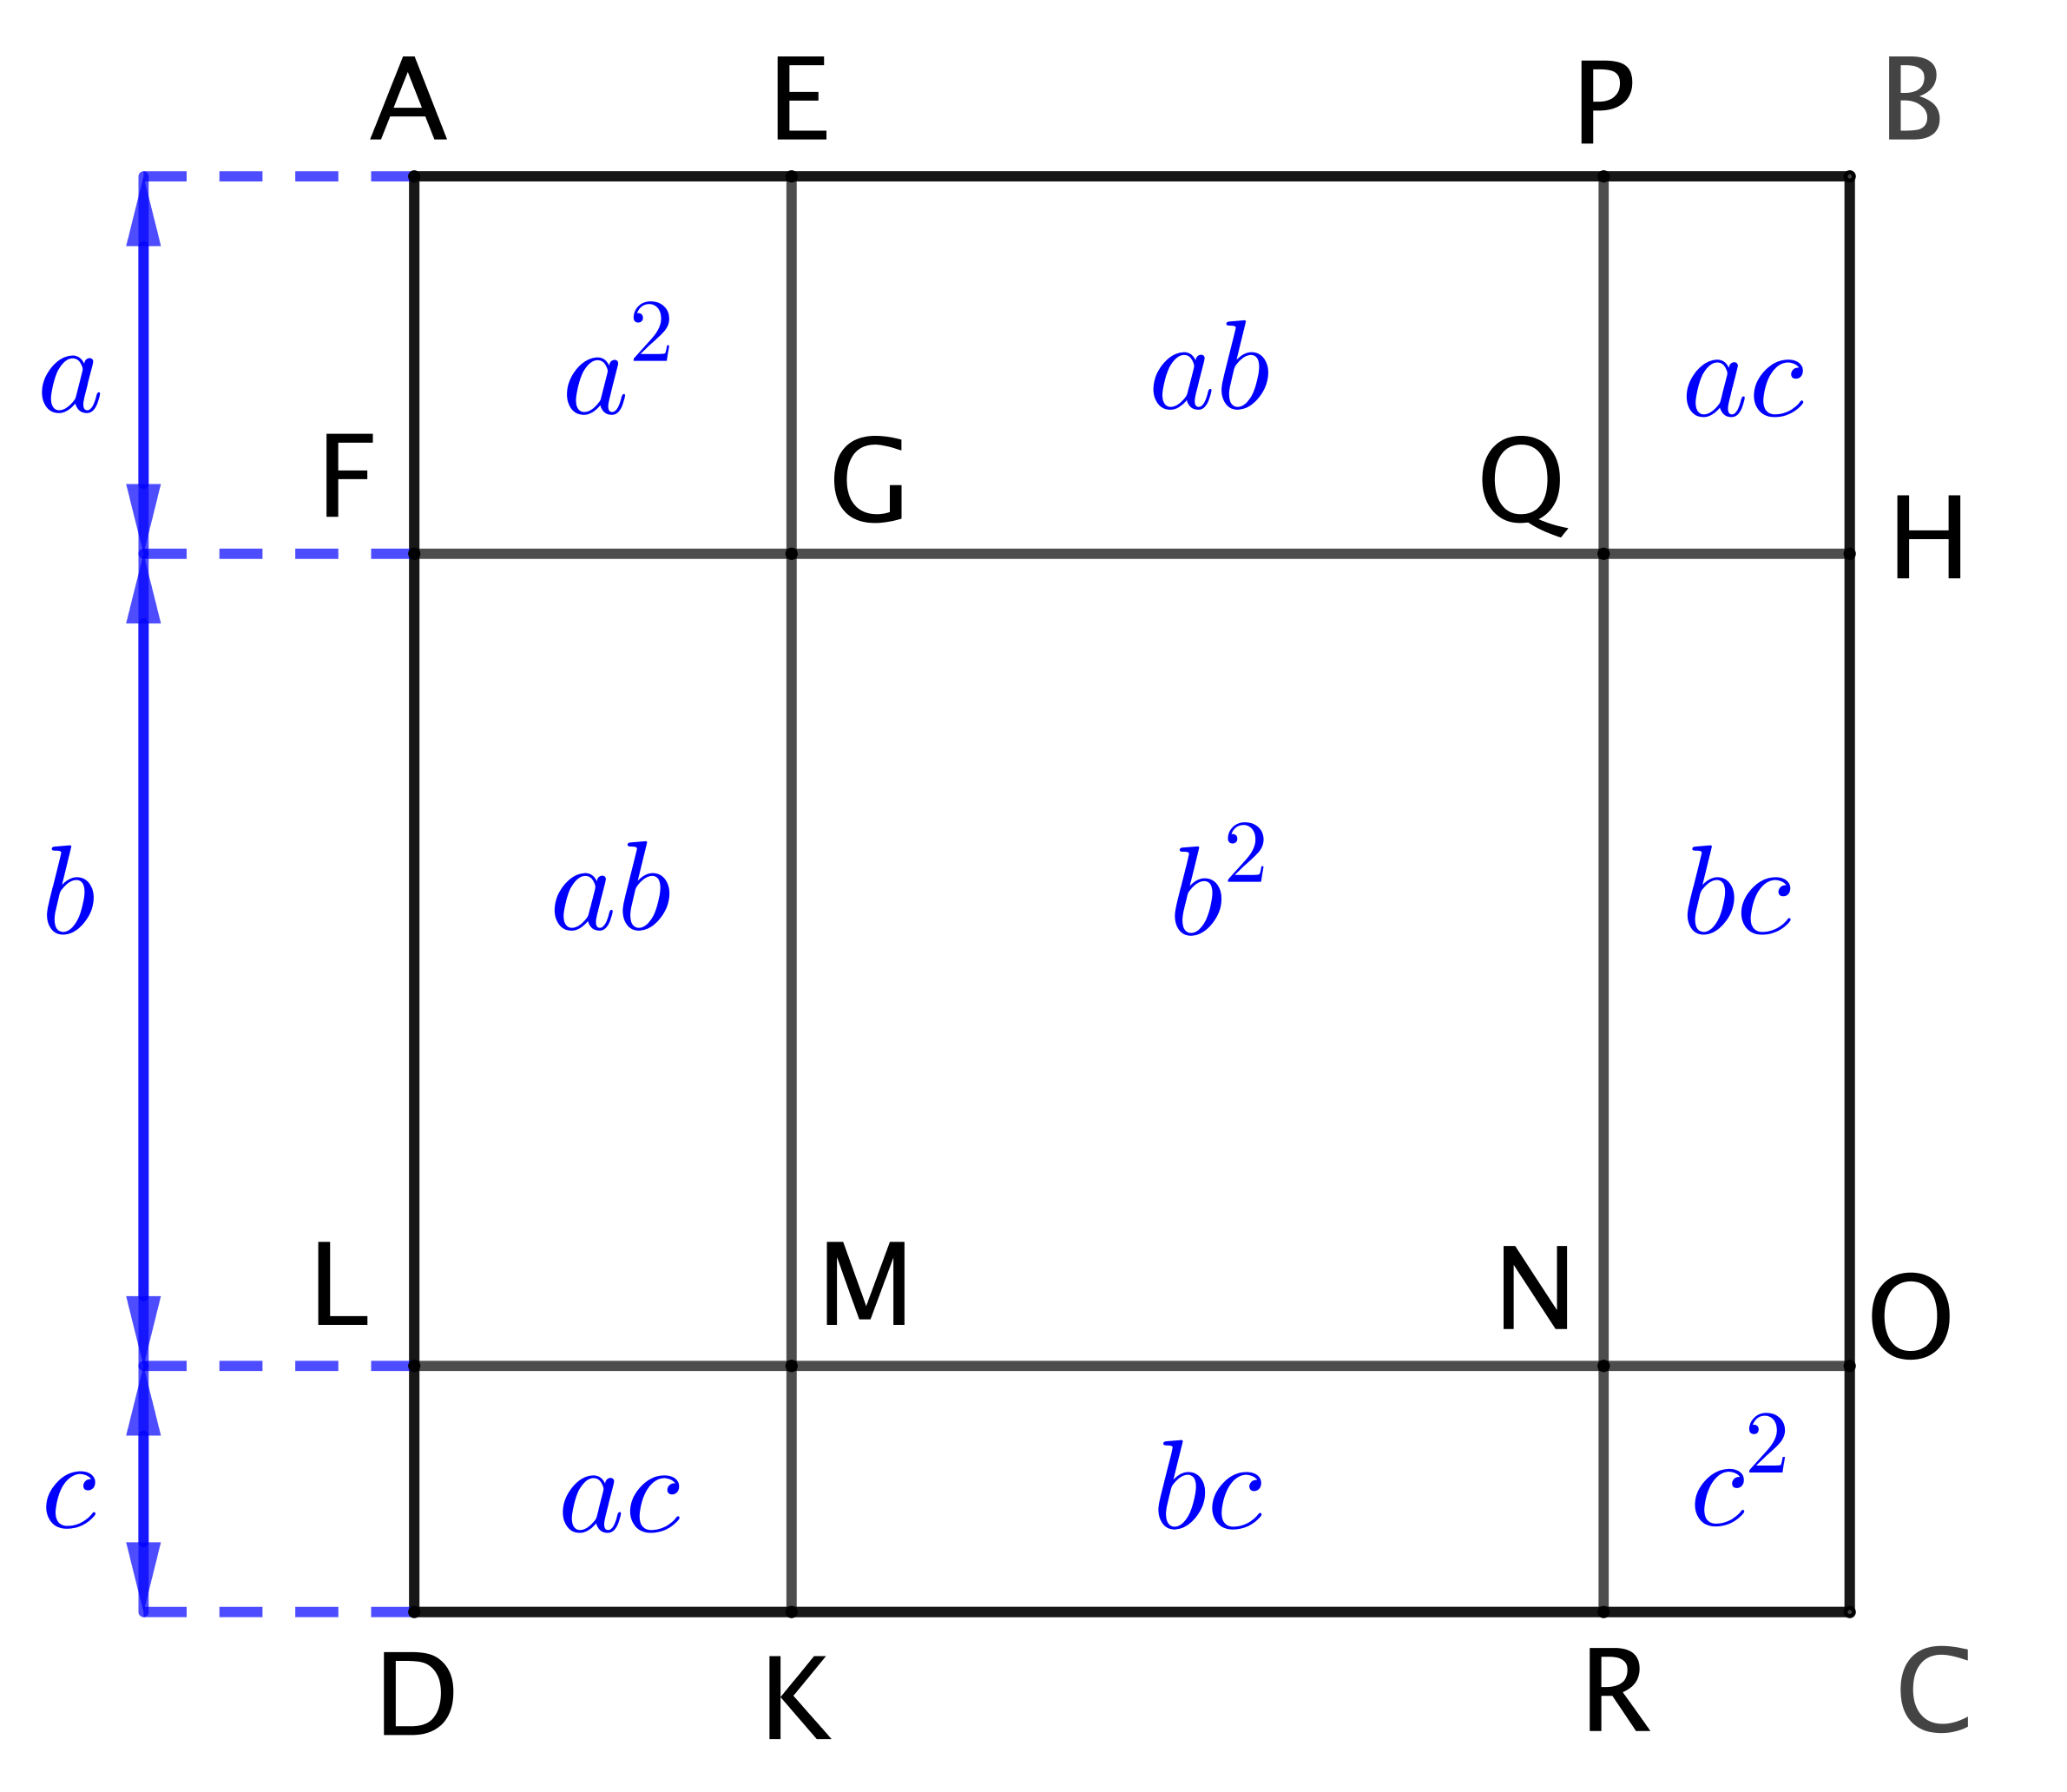
\includegraphics[scale = .7]{identities-geo-poly-n-co/areas-n-identities/(a+b)^3.png}}
	\end{center}
	\vspace{-1.25em}
\end{wrapfigure} 

Bien que rigoureuse, la démarche précédente est peu satisfaisante car elle balaye d'un revers de main l'approche géométrique dont le rôle est réduit à la découverte d'une formule.


\medskip

Si l'on considère le dessin ci-contre, il est tout de même dommage de devoir passer par du calcul algébrique, un peu pénible ici, pour avoir l'identité $(a + b + c)^2 = a^2 + b^2 + c^2 + 2 ab + 2 ac + 2 bc$ avec $a$ , $b$ et $c$ des réels de signes quelconques.


\medskip

Ce qui serait bien ce serait de pouvoir dire que puisque $(a + b + c)^2 = a^2 + b^2 + c^2 + 2 ab + 2 ac + 2 bc$ est vraie si $a > 0$ , $b > 0$ et $c > 0$ , alors l'identité est automatiquement vérifiée par $a$ , $b$ et $c$ des réels de signes quelconques.


% ----------- %


\medskip

Ce passage automatique est bien licite car nous avons le fait \ref{poly-nullity-pos} ci-après que l'on peut appliquer aux polynômes suivants.
\begin{itemize}[label=\small\textbullet]
	\item $P(a ; b) = (a + b)^2 - a^2 - b^2 - 2 ab$

	\item $P(a ; b ; c) = (a + b + c)^2 - a^2 - b^2 - c^2 - 2 ab - 2 ac - 2 bc$
\end{itemize}


\medskip

\begin{fact} \label{poly-nullity-pos}
	Soit $P \in \polyset{\RR}{X_1 | ... | X_n}$ un polynôme réel à $n$ variables où $n \in \NNs$ .
	
	\smallskip
	
	Si $P$ s'annule sur $\left( \RRsp \right)^n$ alors $P$ s'annule sur $\RR^n$ tout entier. 
\end{fact}


\begin{proof}
	Faisons une preuve par récurrence sur $n \in \NNs$ pour démontrer la validité de la propriété $\probaset{P}(n)$ définie comme suit :
	\emph{\og 
		Pour tout polynôme réel $P \in \polyset{\RR}{X_1 | ... | X_n}$ à $n$ variables,
		si $P$ s'annule sur $\left( \RRsp \right)^n$ alors $P$ s'annule sur $\RR^n$ tout entier. 
	\fg}.

	\begin{itemize}[label=\small\textbullet]
		\item \emph{Cas de base.}
	
		\noindent
		$\probaset{P}(1)$ signifie qu'un polynôme réel à une variable s'annulant sur $\RRsp$ est identiquement nul sur $\RR$ tout entier.
		
		\smallskip
		\noindent
		Comme un polynôme réel non nul n'a qu'un nombre fini de racines, nous avons la validité de $\probaset{P}(1)$ .


		\medskip
		\item \emph{Hérédité.}
	
		\noindent
		Supposons $\probaset{P}(n)$ valide pour un naturel $n$ fixé, mais quelconque, puis considérons un polynôme $P$ de $(n + 1)$ variables qui vérifie les conditions de la propriété $\probaset{P}(n + 1)$ .
	
		\smallskip
		\noindent
		Fixons $x \in \RRsp$ et considérons le polynôme $P_x(X_1 ; ... ; X_n) = P(X_1 ; ... ; X_n ; x)$ .
		Comme $P_x$  vérifie les conditions de la propriété $\probaset{P}(n)$ ,
		nous avons par hypothèse de récurrence 
		$P_x(x_1 ; ... ; x_n) = 0$ soit $P(x_1 ; ... ; x_n ; x) = 0$ pour tous réels $x_1$ , ... , $x_n$ .
	
		\smallskip
		\noindent
		Fixons maintenant des réels $x_1$ , ... , $x_n$ de signes quelconques et considérons le polynôme $p(X) = P(x_1 ; ... ; x_n ; X)$ .
		Comme $p$ vérifie $\probaset{P}(1)$ , nous avons $p(x) = 0$ soit $P(x_1 ; ... ; x_n ; x) = 0$ pour tout réel $x$ .
	
		\smallskip
		\noindent
		Finalement $P(x_1 ; ... ; x_n ; x) = 0$ pour tous réels $x_1$ , ... , $x_n$ , $x$ .
		Nous avons bien déduit la validité de $\probaset{P}(n+1)$ à partir de celle de $\probaset{P}(n)$ .


	\medskip
	\item \emph{Conclusion.}
	
	\smallskip
	\noindent
	Par récurrence sur $n \in \NNs$ , la propriété $\probaset{P}(n)$ est vraie pour tout naturel non nul $n$ .
	\end{itemize}
\end{proof}


% ----------- %


\begin{example}
	En utilisant une approche géométrique semblable à celle présentée plus haut, il devient évident, mais aussi rigoureux maintenant, d'affirmer que pour tous réels $a_1$ , ... , $a_n$ , où $n \in \NNs$ , l'on a :
\[
	\left( \sum_{k=1}^{n}a_k \right)^2
	=
	\sum_{k=1}^{n} \left( a_k \right)^2
	+
	2 \sum_{1 \leq i < j \leq n} a_i a_j
\]
\end{example}


% ----------- %


\begin{example}
	Nous laissons le soin au lecteur de vérifier à l'aide d'un cube, le solide géométrique, l'identité $(a + b)^3 = a^3 + 3 a^2 b + 3 a b^2 + b^3$ valable pour tous réels $a$ et $b$ .
\end{example}


% ----------- %


\medskip


\begin{wrapfigure}{r}{0.45\textwidth} 
	\vspace{-.5em}
	\begin{center}
		\fbox{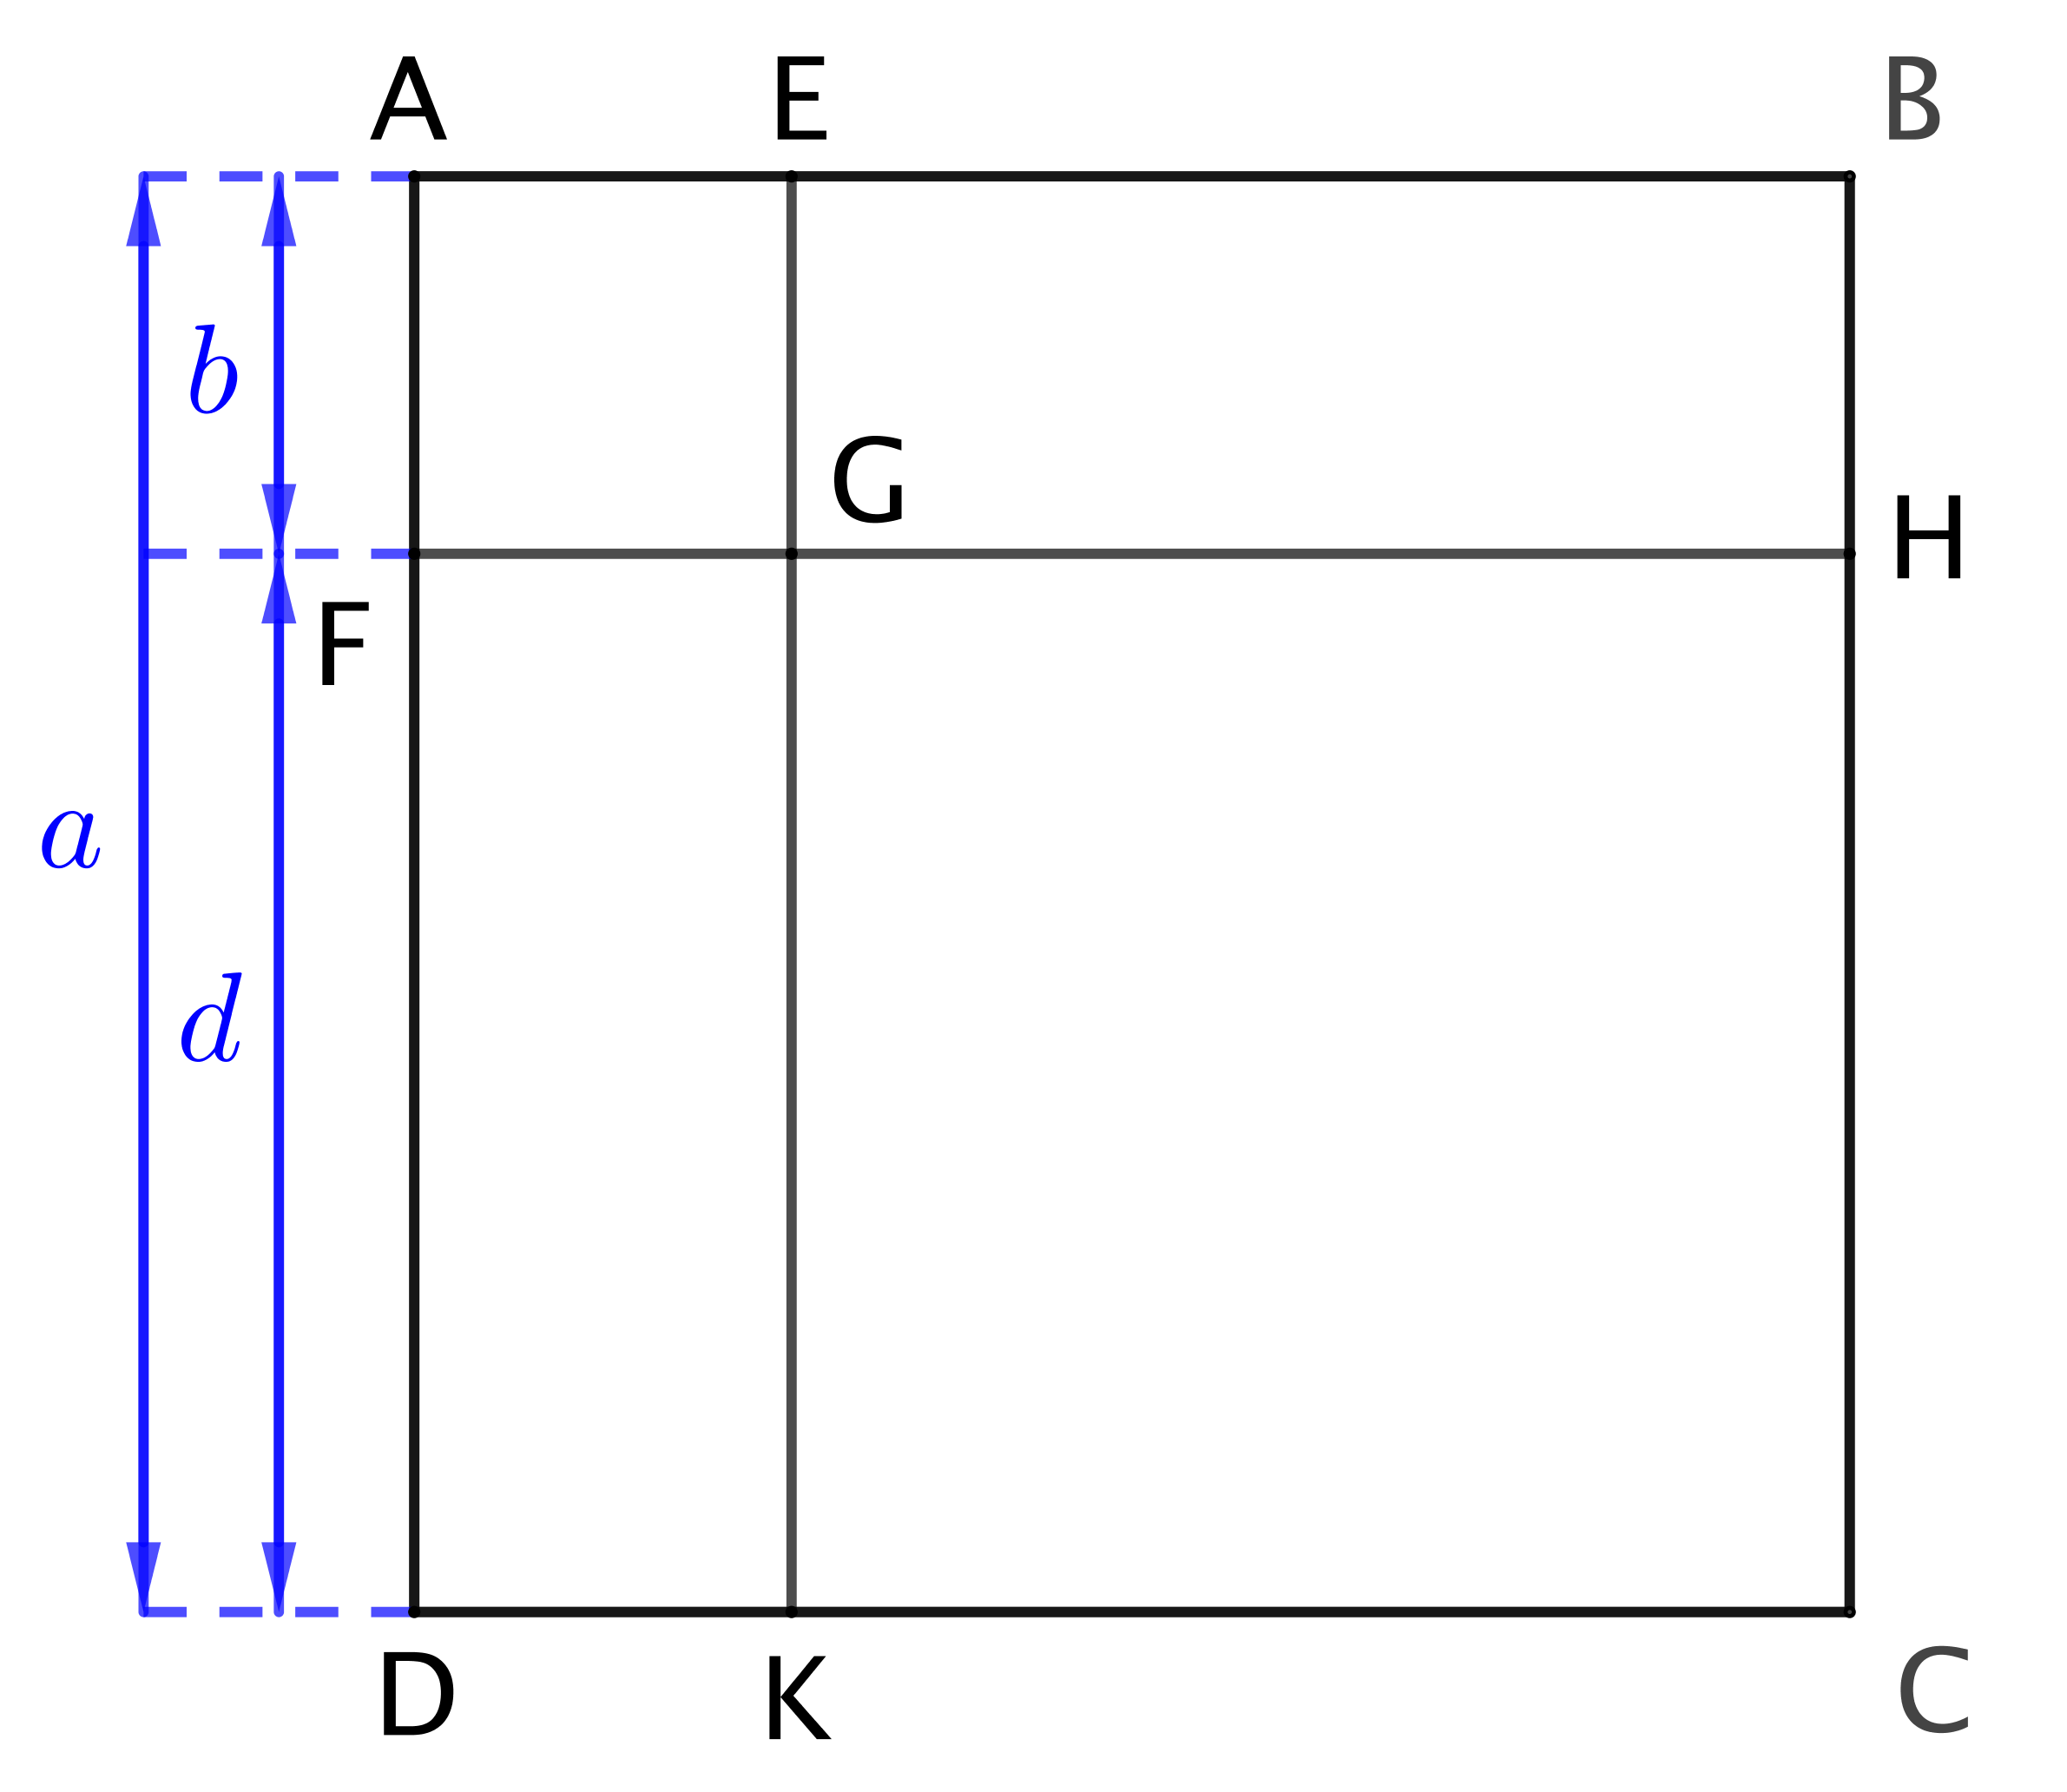
\includegraphics[scale = .7]{/areas-n-identities/(a-b)^2.png}}
	\end{center}
	\vspace{-1.25em}
\end{wrapfigure} 


Considérons maintenant le dessin ci-contre avec $d = a - b$ et la contrainte $a > b$ . Le fait \ref{poly-nullity-pos}, bien que très utile, ne peut plus s'appliquer ici bien que nous ayons le calcul géométrique évident suivant.

\smallskip

$\geoset*{A}{GHCK} = \geoset*{A}{ABCD} - \geoset*{A}{ABHF} - \geoset*{A}{AEKD} + \geoset*{A}{AEGF}$
	
\smallskip
	
$(a-b)^2 = a^2 - 2ab + b^2$


\medskip

Comment faire alors pour en déduire que pour tous réels $a$ et $b$ , l'identité $(a - b)^2 = a^2 + b^2 - 2ab$ reste valable ?
Aucune crainte à avoir car nous disposons du fait \ref{poly-nullity-interval} moins restrictif suivant. 


\medskip

\begin{fact} \label{poly-nullity-interval}
	Soit $P \in \polyset{\RR}{X_1 | ... | X_n}$ un polynôme réel à $n$ variables où $n \in \NNs$ .
	
	\smallskip
	
	Si $\geoset{E} \subseteq \RR^n$ contient $\geoset*{E}{1} \times \cdots \times \geoset*{E}{n}$ où chaque $\geoset*{E}{k} \subseteq \RR$ est infini,
	et si $P$ s'annule sur $\geoset{E}$ alors $P$ s'annule sur $\RR^n$ tout entier. 
\end{fact}


\begin{proof}
	Il est très facile de vérifier que la preuve du fait \ref{poly-nullity-pos} s'adapte au cadre plus général proposé ici.
\end{proof}


% ----------- %


\medskip

\begin{example}
Considérons le dessin ci-dessous avec $d = a - b$ et la contrainte $a > b$ afin d'établir l'identité $(a+b)(a-b) = a^2 - b^2$ .


\smallskip

\begin{center}
	\fbox{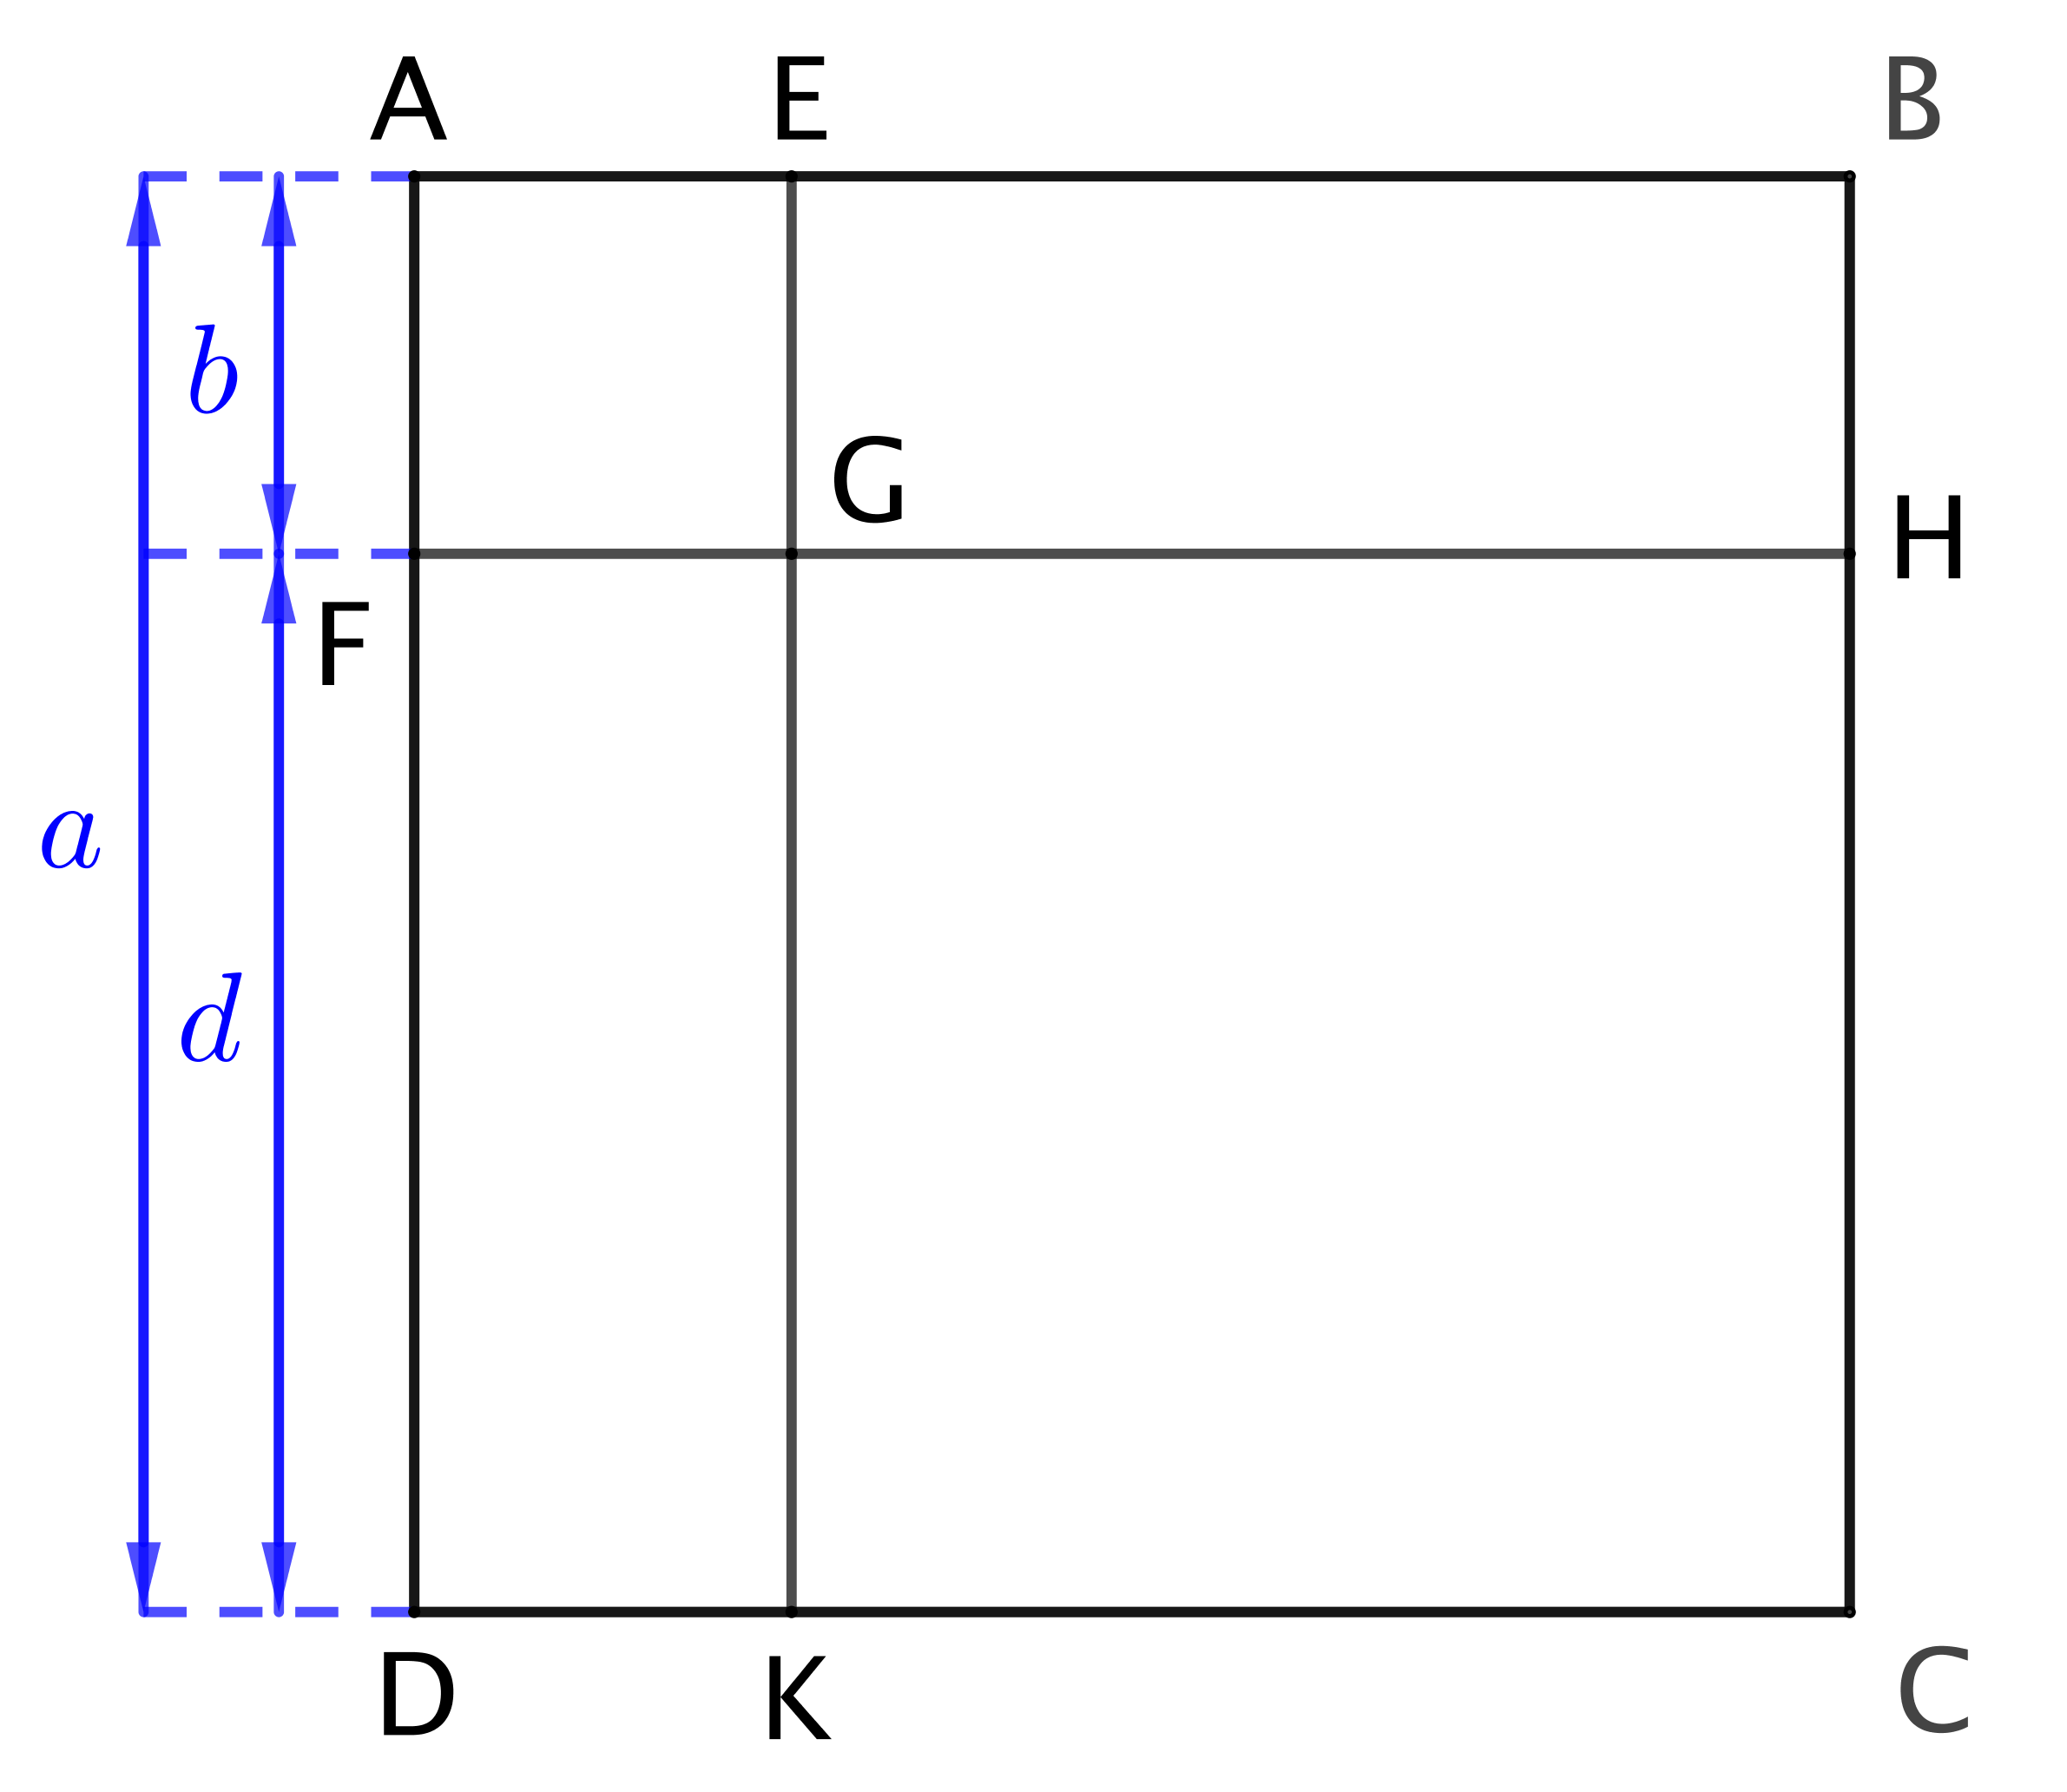
\includegraphics[scale = .7]{/areas-n-identities/(a-b)^2.png}}
\end{center}


\medskip


Commençons par des calculs géométriques simples.

\smallskip
	
$\geoset*{A}{ABCD} - \geoset*{A}{AEGF} = \geoset*{A}{GHCK} + \geoset*{A}{EBHG} + \geoset*{A}{FGKD}$
	
\smallskip
	
$a^2 - b^2 = \geoset*{A}{GHCK} + \geoset*{A}{EBHG} + \geoset*{A}{FGKD}$


\medskip

En déplaçant ensuite le rectangle $EBHG$ comme ci-dessous, nous obtenons alors un rectangle de dimension $(a+b) \times (a-b)$ . 
	

\smallskip

\begin{center}
	\fbox{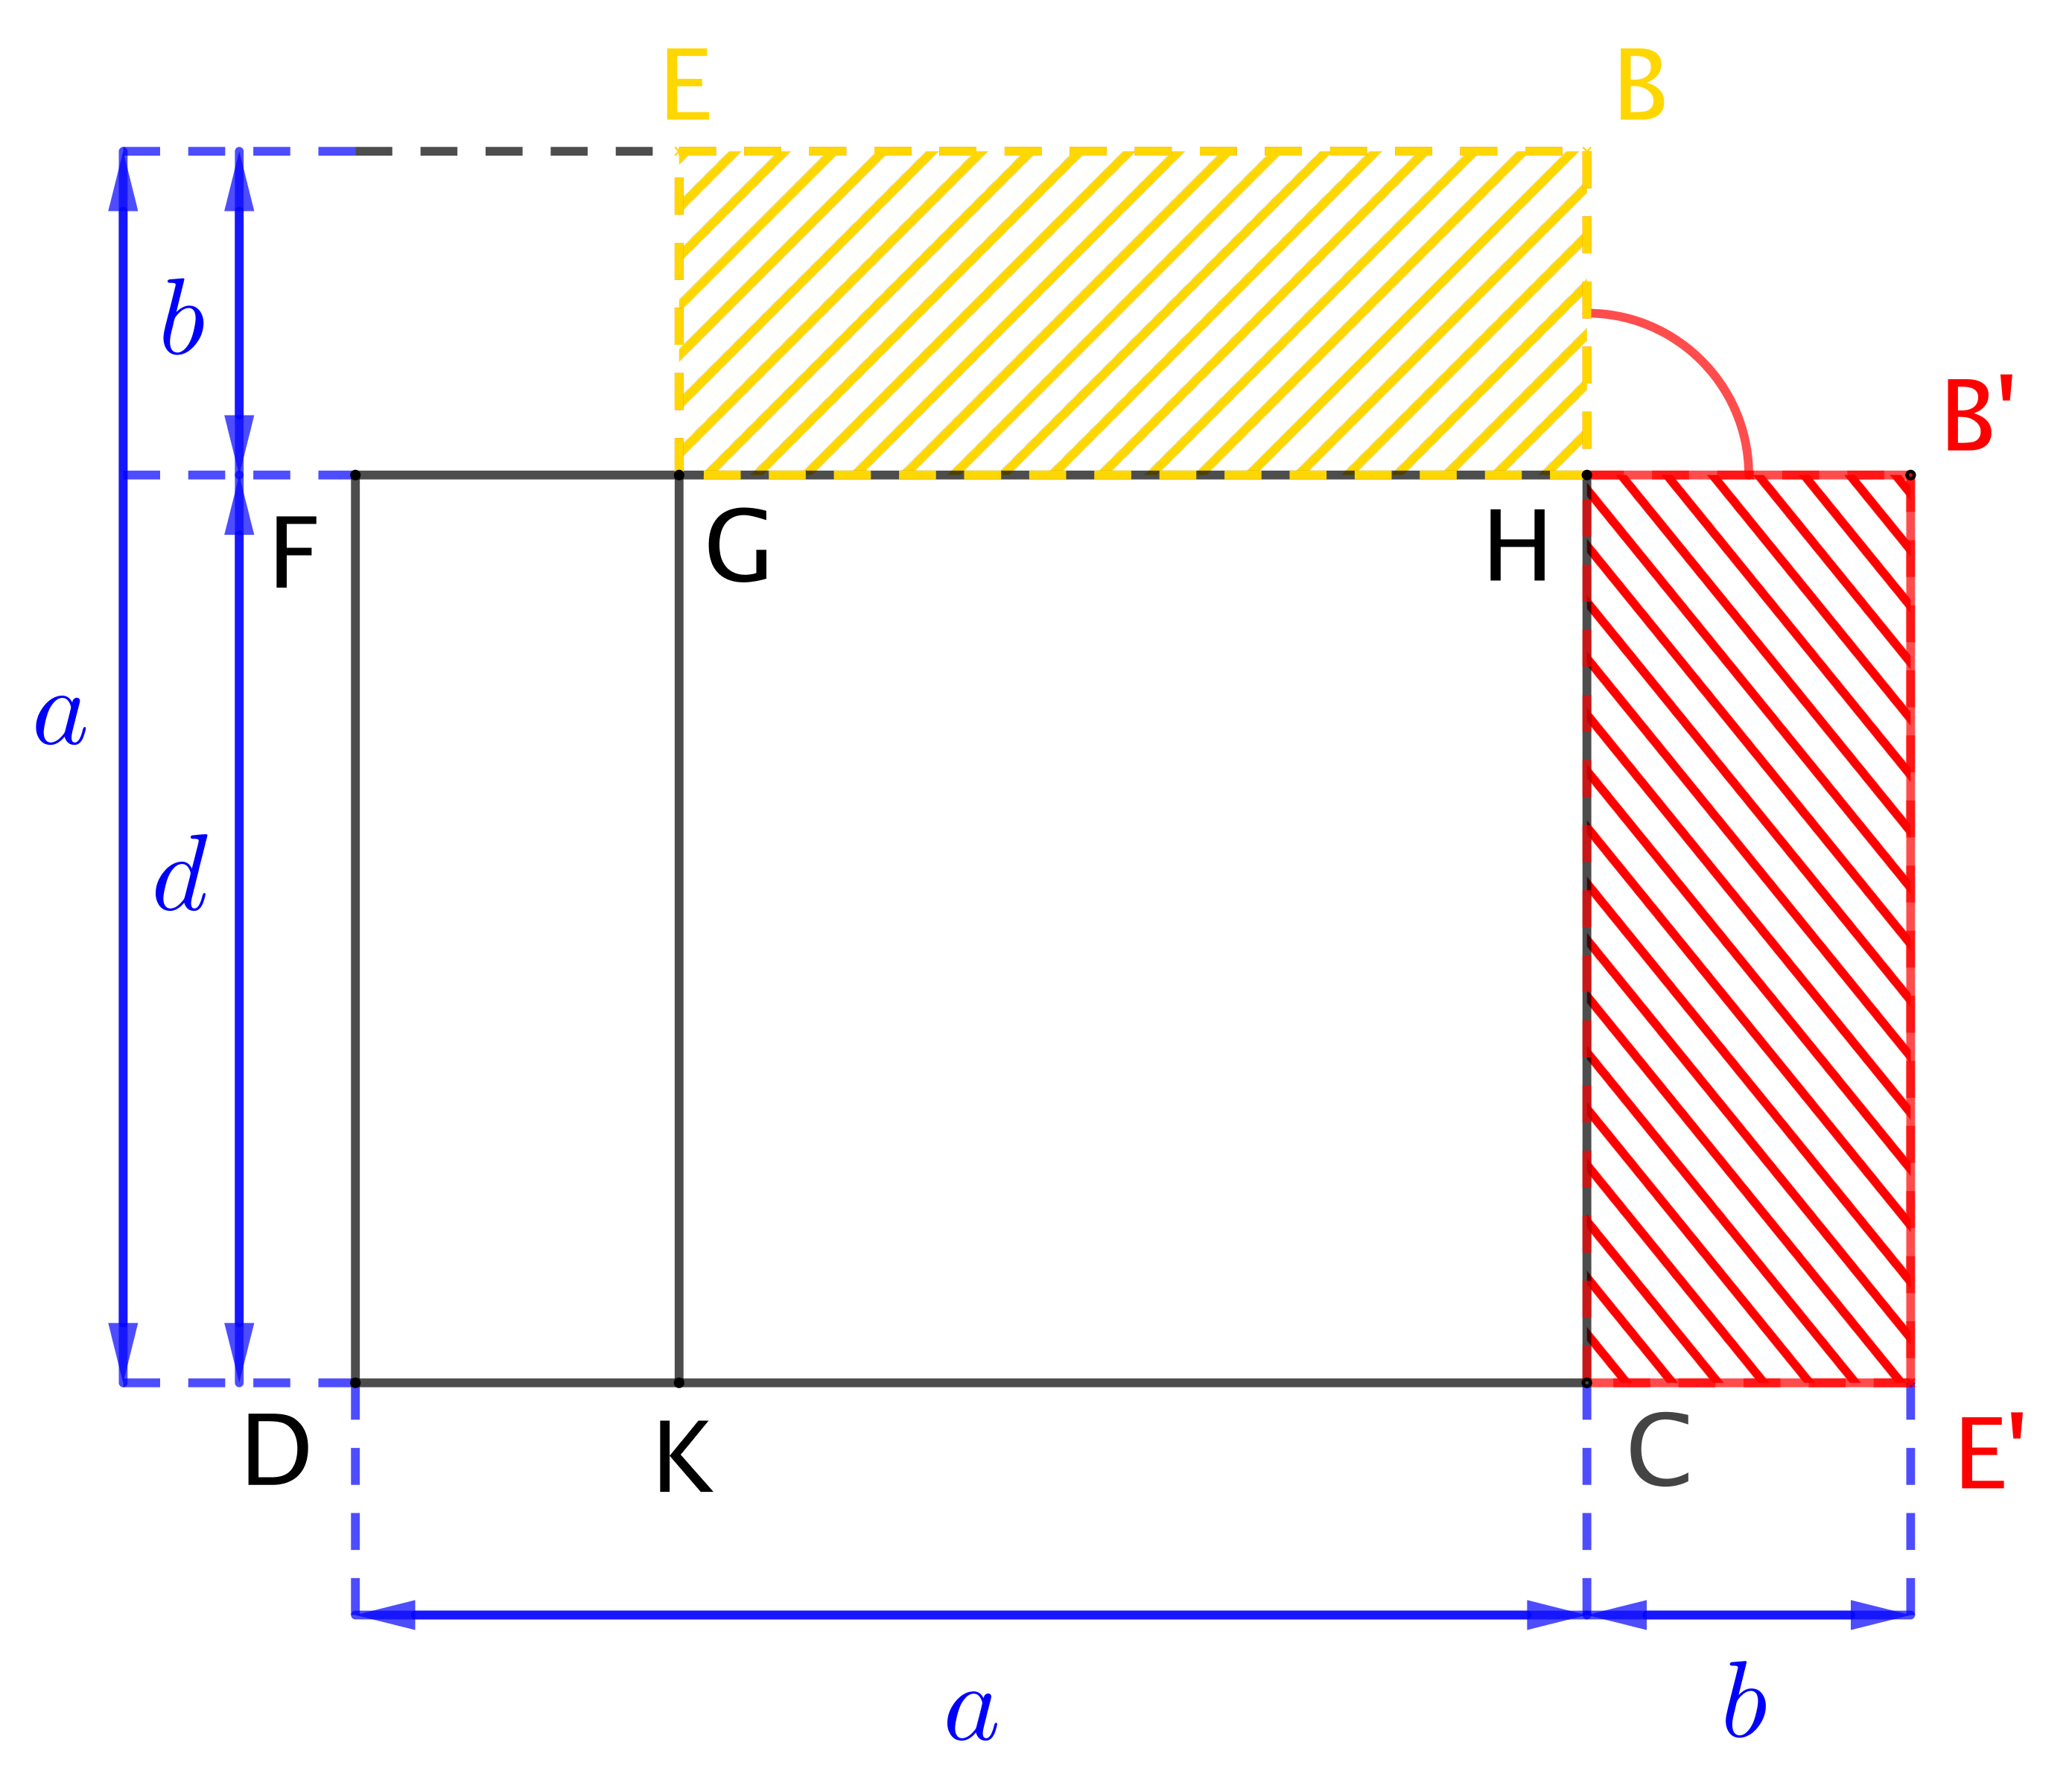
\includegraphics[scale = .7]{/areas-n-identities/(a-b)(a-b)-spe.png}}
\end{center}


\medskip

Finalement, nous obtenons $a^2 - b^2 = (a+b)(a-b)$ si $a > b$ .
Le fait \ref{poly-nullity-interval} permet alors d'affirmer que $\forall (a ;b) \in \RR^2$, $a^2 - b^2 = (a+b)(a-b)$ .
\end{example}
